\newcommand{\lecturetitle}[1]{
  \title{01204211 Discrete Mathematics \\ #1}
  \author{Jittat Fakcharoenphol}
  \frame{\titlepage}
}

\lecturetitle{Lecture 8: Mathematical Induction 3}

\begin{frame}\frametitle{Review: Mathematical Induction}
  \begin{tcolorbox}
    Suppose that you want to prove that property $P(n)$ is true for
    every natural number $n$.\\
    
    Suppose that we can prove the following two facts:
    
    {\bf Base case:} $P(1)$ \\
    {\bf Inductive step:} For any $k\geq 1$, $P(k)\Rightarrow P(k+1)$ \\
    
    The {\bf Principle of Mathematical Induction} states that $P(n)$
    is true for every natural number $n$.
  \end{tcolorbox}

  The assumption $P(k)$ in the inductive step is usually referred to
  as {\bf the Induction Hypothesis}.
\end{frame}

\begin{frame}\frametitle{The Induction Hypothesis}
  \begin{theorem}
    For any integer $n\geq 1$, $\frac{1}{1^2} + \frac{1}{2^2} + \frac{1}{3^2} + \cdots +\frac{1}{n^2} < 2$.
  \end{theorem}
  \pause
  \begin{proof}
    The statement $P(n)$ that we want to prove is ``$\frac{1}{1^2} + \frac{1}{2^2} + \frac{1}{3^2} + \cdots +\frac{1}{n^2} < 2$''.
    
    \pause
    \vspace{0.1in}

    {\bf Case case:} For $n=1$, the statement is true because $1<2$.

    \pause
    \vspace{0.1in}
    
    {\bf Inductive step:} For $k\geq 1$, let's assume $P(k)$ and we prove that $P(k+1)$ is true.

    \pause

    The induction hypothesis is: $\frac{1}{1^2} + \frac{1}{2^2} + \frac{1}{3^2} + \cdots +\frac{1}{k^2} < 2$.

    We want to show $P(k+1)$, i.e., $\frac{1}{1^2} + \frac{1}{2^2} + \frac{1}{3^2} + \cdots +\frac{1}{k^2}+\frac{1}{(k+1)^2} < 2$.

    Then...
  \end{proof}
\end{frame}

\begin{frame}\frametitle{Strengtening the Induction Hypothesis (1)}
  \begin{itemize}
  \item
    Is the assumption
    \[ \frac{1}{1^2} + \frac{1}{2^2} + \frac{1}{3^2} + \cdots +\frac{1}{k^2} < 2.\]
    ``strong'' enough to prove
    \[ \frac{1}{1^2} + \frac{1}{2^2} + \frac{1}{3^2} + \cdots +\frac{1}{k^2}+\frac{1}{(k+1)^2} < 2 \ \ ?\]

    Why?
    \pause
    
  \item To prove $P(k+1)$, we need a ``gap'' between the LHS and 2, so
    that we can add $1/(k+1)$ without blowing up the RHS.
  \end{itemize}
\end{frame}

\begin{frame}\frametitle{Strengtening the Induction Hypothesis (2)}
  \begin{itemize}
  \item Let's see a few values of the sum:
    \begin{itemize}
    \item $1/1 = 1.$ \pause
    \item $1/1 + 1/4 = 1.25.$ \pause
    \item $1/1 + 1/4 + 1/9 \approx 1.361.$ \pause
    \item $1/1 + 1/4 + 1/9 + 1/16 \approx 1.4236.$ \pause
    \item $1/1 + 1/4 + 1/9 + 1/16 + 1/25 \approx 1.4636.$
    \end{itemize}
    Yes, there is a gap.  But how large?
    \pause
    
  \item We need the gap to be large enough to insert $1/(k+1)^2$.
    \pause
  \item After a ``mysterious'' moment, we observe that
    \[ \frac{1}{1^2} + \frac{1}{2^2} + \frac{1}{3^2} + \cdots +\frac{1}{n^2} < 2 - \frac{1}{n}.\]
  \end{itemize}
\end{frame}

\begin{frame}\frametitle{Strengtening the Induction Hypothesis (3)}
  \begin{theorem}
    For any integer $n\geq 1$, $\frac{1}{1^2} + \frac{1}{2^2} + \frac{1}{3^2} + \cdots +\frac{1}{n^2} < 2 - \frac{1}{n}$.
  \end{theorem}
  \pause
  \begin{proof}
    {\footnotesize
      (... the beginning is left out ...)
      
      {\bf Inductive step:} For $k\geq 1$, assume that $ \frac{1}{1^2} + \frac{1}{2^2} + \frac{1}{3^2} + \cdots +\frac{1}{k^2} < 2 - \frac{1}{k}. $
      
      Adding $1/(k+1)^2$ on both sides, we get
      \begin{eqnarray*}
        \frac{1}{1^2} + \frac{1}{2^2} + \frac{1}{3^2} + \cdots +\frac{1}{k^2}+\frac{1}{(k+1)^2}
        &<& 2 - \frac{1}{k} +\frac{1}{(k+1)^2} \\
        &=& 2 - \left(\frac{(k+1)^2 - k}{k(k+1)^2}\right).
      \end{eqnarray*}
      Since one can verify that $\frac{(k+1)^2 - k}{k(k+1)^2} >
      \frac{1}{k+1}$, we conclude that
      \[
      \frac{1}{1^2} + \frac{1}{2^2} + \frac{1}{3^2} + \cdots +\frac{1}{k^2}+\frac{1}{(k+1)^2} < 2 - \frac{1}{k+1},
      \]
      as required.
    }
  \end{proof}
\end{frame}

\begin{frame}\frametitle{L-shaped tiles}
  A 4x4 area with a hole in the middle can be tiled with L-shaped tiles.

  \vspace{0.2in}
  
  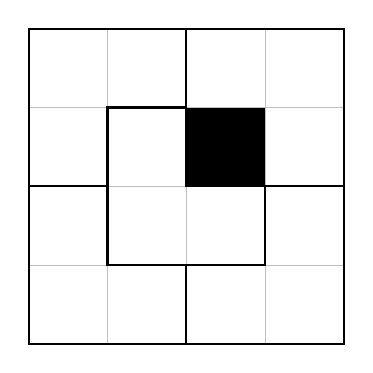
\begin{tikzpicture}
    \draw[step=1cm,lightgray,very thin] (0,0) grid (4,4);
    \draw[thick] (0,0) -- (0,2) -- (1,2) -- (1,1) -- (2,1) -- (2,0) -- cycle;
    \fill[black] (2,2) -- (2,3) -- (3,3) -- (3,2) -- cycle;
    \draw[thick] (0,2) -- (0,4) -- (2,4) -- (2,3) -- (1,3) -- (1,2) -- cycle;
    \draw[thick] (1,1) -- (1,3) -- (2,3) -- (2,2) -- (3,2) -- (3,1) -- cycle;
    \draw[thick] (2,2) rectangle (4,4);
    \draw[thick] (4,2) -- (4,0) -- (2,0);
  \end{tikzpicture}

  \vspace{0.1in}

  This is true for 2x2 area, 8x8 area, even 16x16 area. \pause

  \vspace{0.1in}

  This motivates us to try to prove that it is possible to use
  L-shaped tiles to tile a $2^n\times 2^n$ area.
\end{frame}

